\section{Обзор существующих работ и решений}
\label{section.3}
\subsection{Маркетплейсы}
На данный момент существует большое количество NFT маркетплейсов: opensea\cite{opensea}, rarible\cite{rarible}, solanart\cite{solanart}. Если брать маркетплейсы только на базе NEAR Protocol, тогда существуют такие примеры как: Paras\cite{paras}, Mintbase\cite{mintbase}. Остановимся на них поподробнее.

\paragraph{Paras}

Paras является наиболее популярным, интерфейс взаимодействия представлен пользователю в веб-браузере по адресу paras.id. Для того, чтобы авторизоваться нужно использовать
предоставить свой NEAR кошелек. Paras предоставляет огромное количество функций:
\begin{enumerate}
    \item Создать NFT токен.
    \item Выставить на продажу NFT токен.
    \item Обновить цену выставленному на продажу NFT токену.
    \item Убрать с продажи выставленной NFT токен.
    \item Уничтожить свой NFT токен.
    \item Получить продаваемые NFT токены со следующей фильтрацией:
        \begin{enumerate}
            \item Фильтрация по содержимому токена(картинке) - пиксель арт, фотографии, иллюстрации и так далее.
            \item Фильтрация по времени создания.
            \item Фильтрация по максимальной цене.
            \item Фильтрация по минимальной цене.
        \end{enumerate}
    \item Выставить оффер на непродаваемый токен.
\end{enumerate}

Smart-контракты Paras лежат в открытом доступе\cite{parasnftcontract, parasmarketplacecontract}.

\begin{remark}
    Обычно smart-контракты DApps принято выкладывать в открытый доступ, чтобы любой пользователь мог их посмотреть и полностью доверять сервису.
\end{remark}

С точки зрения написания smart-контрактов Paras имеет абсолютно такую же структуру NFT smart-контракта, потому что они придерживаются стандарта \cite{nftstandart}(см. \hyperref[section.4.1]{\color{blue} 4.1}).
Дополнительно они привязывают каждый токен к какой-то конкретной коллекции и не позволяют создавать токен без привязки к коллекции.
Схема выглядит таким образом \hyperref[img.parascollections]{\color{blue} 3.1}:

\begin{figure}[H]
	\centering
	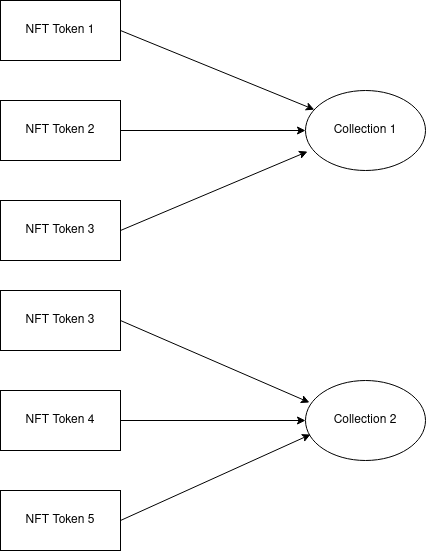
\includegraphics[height=60mm]{fig/parascollections.png}
	\caption{NFT токены и колекции в paras}
    \label{img.parascollections}
\end{figure}

Smart-контракт маркетплейса paras предоставляет дополнительную функцию, как выставление оффера(предложения о покупке) на любой NFT токен. Эту функцию мы планируем позаимствовать в ближайшем будущем.

% \begin{listing}
% \begin{minted}[breaklines,fontsize=\scriptsize]{js}
% {
%     token_id: "304990:24",TokenSeriesJson
%     owner_id: "maxzeinly.near",
%     metadata: {
%         title: "Proof of Attendance No.1 #24",
%         description: null,
%         media: "bafybeib3c3r7vjbmyetawahj4kprei6satcrq23k2qjlx2gnmxmv5c6lza",
%         media_hash: null,
%         copies: 1111,
%         issued_at: "1652813800358071368",
%         expires_at: null,
%         starts_at: null,
%         updated_at: null,
%         extra: null,
%         reference: "bafkreiai54itp2hf267leg6754xmlst6j5m3yp3sin6n5bgva2q44wwtem",
%         reference_hash: null
%     },
%     approved_account_ids: {}
% }
% \end{minted}
% \caption{Структура NFT}
% \end{listing}

Paras, как и большинство маркетплейсов хранит медиа-файл и метаданные NFT на IPFS\cite{ipfs}(см. \hyperref[section.5.1.5]{\color{blue} 5.1.5}). IPFS предоставляется сервисом fleek\cite{fleek}. В качестве ссылки на медиа-файл и метаданные они хранят CID, а не полный URL, это связанно с тем, что минт NFT таким образом будет гораздо дешевле, ведь хранение в NEAR, довольно дорогое(см. \hyperref[section.5.1.4]{\color{blue} 5.1.4}). Но есть и минус этой экономии, на NEAR Wallet, скорее всего это изображение не будет отображаться, так как NEAR Wallet, при не указании протокола соединения, будет подставлять CID не в шлюз IPFS от fleek (Листинг \hyperref[lst.pastecidnearwallet]{\color{blue} 1}), а доступность и скорость получения контента зависят от шлюза.

\begin{listing}[H]
\begin{minted}[breaklines,fontsize=\scriptsize]{js}
function buildMediaUrl(media, base_uri) {
    if (!media || media.includes('://') || media.startsWith('data:image')) {
        return media;
    }
    if (base_uri) {
        return `${base_uri}/${media}`;
    }
    return `https://cloudflare-ipfs.com/ipfs/${media}`;
}
\end{minted}
\caption{Подстановка CID в URL у NEAR Wallet\cite{pastecidnearwallet}}
\label{lst.pastecidnearwallet}
\end{listing}

Давайте рассмотрим структуру метаданных NFT (Листинг \hyperref[lst.parasnftmetadatastruct]{\color{blue} 2}). Paras, хоть и поддерживает по стандарту NEP-171 поле <<description>>, но хранит описание в метаданных NFT токена. Это аналогично тем же причинам, что и при хранении CID, а не полного URL в полях на медиа-файл и метаданные. Также они хранят название и идентификатор коллекции, создателя NFT, атрибуты и тип файла. Во многом наши метаданные будут подражать этой структуре.

\begin{listing}[H]
\begin{minted}[breaklines,fontsize=\scriptsize]{json}
{
    "description":"Proof of Attendance to events hosted by NEAR Gang Couture.",
    "collection":"Haute Gang - Collaborations",
    "collection_id":"haute-gang-collaborations-by-neargangcouturenear",
    "creator_id":"neargangcouture.near",
    "attributes":[
        {"trait_type":"Rarity","value":"No Star"},
        {"trait_type":"Type","value":"Mask"}
    ],
    "blurhash":"UqFtJxPWpdyDGJ${t2V[?[ICMyenPCxVobae",
    "mime_type":"image/jpeg"
}
\end{minted}
\caption{Структура метаданных NFT в Paras}
\label{lst.parasnftmetadatastruct}
\end{listing}


\paragraph{Mintbase}

Mintbase является менее популярным маркетплейсом, однако он предоставляем гораздо больше категорий NFT, но все ключевые функции такие же. В качестве новых категорий выступают: 3D изображение, gif, профессиональные фотографии, аудиодорожки, произведения художников.

Smart-контракты Mintbase на половину открыты(некоторые в открытом доступе, некоторые нет)\cite{mintbasecontracts}.

// TODO контракты

\subsection{Генеративно-состязательные сети}
